\section{Regression Evaluation}
\begin{multicols}{2}

We saw that for classification, because there were some scenarios like medical diagnostics predictions or costumer facing web site features, where the consequences of false positive were very different than false negatives. It made sense to distinguish these types of errors and do a more detailed analysis. In evaluating classifiers for example we looked at plots like precision recall curves that could show the trade offs a classifier could achieve between making errors of those two types. 

In theory, we could apply the same type of error analysis and more detailed evaluation to regression that we applied for classification. 

For example, we could analyze the regression model's predictions, and categorize errors of one type. Where the regression model's predicted value was much larger than the target value. Compared to a second error type, where the predicted value was much smaller than the target value. 

In practice though it turns out that for most applications of regression, distinguishing between these types of different errors is not as important. 
This simplifies evaluation for regression quite a bit. 

\subsection{$R^2$ score}

In most cases, the default $R^2$ score that's available for regression and psychic learn and that summarizes how well future instances will be predicted. It's adequate for most tasks. 

As a reminder, the $R^2$ score for \emph{perfect predictor} is \textbf{1.0}. And for a predictor that always output the \emph{same constant value}, the $R^2$ score is \textbf{0.0}. 

The $R^2$ score despite the squared in the name that suggests it's always positive does have the potential to go \emph{negative} for bad model fits, such as when fitting non-linear functions to data. 

\subsection{Alternative metrics}

There are a few alternative regression evaluation metrics you should be aware of that work differently than the $R^2$ score. 

\subsubsection{Mean absolute error}

Mean absolute error takes the mean absolute difference between the target and predicted values. In machine running terms this corresponds to the expected value of L1 norm laws. This is sometimes used for example to asses focused outcomes for regression in time series analysis. 

\subsubsection{Mean squared  error}
Mean squared error takes the mean squared difference between the target and predicted values and this corresponds to the expected value of the L2 norm loss. This is widely used for many regression problems and larger errors have correspondingly larger squared contributions to the mean error. 

Like mean absolute error, mean squared error doesn't distinguish between over and under estimates. 

\subsubsection{Median absolute error}

Finally one situation that does arise quite often, is the existence of \emph{outliers} in the data, which can have unwanted influence on the overall $R^2$ or mean squared value. So in those cases, when ignoring outlier is important, you can use the \emph{median} absolute error score, which is robust with the presence of outliers because it uses the median of the error distribution rather than the mean. 

\subsection{Dummy Regressors}

We saw how using how dummy classifiers could give us simple but useful baselines to compared against when evaluating a classifier. The same functionality exist for regression. 

DummyRegressors, as you might guess, are the counterpart to DummyClassifiers for regression. And they serve a similar role as a null outcome baseline and sanity check for regression models. Since regression models have continuous value prediction outputs. The strategy parameter for DummyRegressors gives you a choice of function that you can apply to the distribution of target values found in the training set. You can ask for the mean or median value of the training set targets. The value corresponding to the quantile that you provide or a custom constant value. 

There's a dummy regressor class that provides predictions using simple strategies that do not look at the input data.
 
\begin{center}
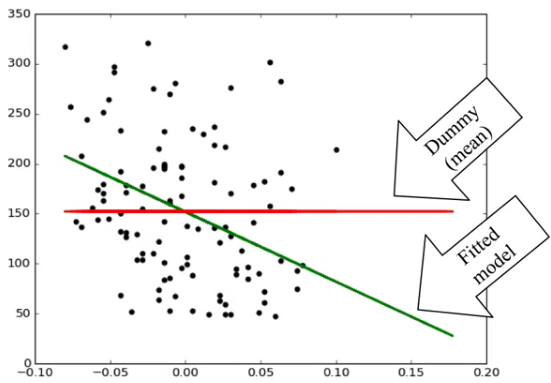
\includegraphics[width=\linewidth]{img/Dummy-Regressor.png}
\end{center}

This example which is available as the regression example from this lecture's notebook shows a scatter plot using database on a single input variable, which is plotted along the x axis from the diabetes data set. 

The points are the data instances from the test split and form a cloud that looks like it may trend down slightly to the right. 

The green line, which is also labeled fitted model is the default linear regression that was fit to the training points. We can see that it’s not a particularly strong fit to the test data. 

The red line labeled dummy mean, shows a linear model that uses the strategy of always predicting the mean of the training data. 

So this is an example of a dummy regressor. 

You can look at the notebook to see that a dummy regressor is created and used just like a regular regression model. You create, fit with the training data, and then call predict on the test data. Although again, like the dummy classifier you \emph{should not} use the dummy regressor for actual problems. Its only use is to provide a baseline for comparison. 

Looking at the regression metrics output from the linear model compared to the dummy model. 

\begin{verbatim}
Linear model, coefficients:[-698.80206267]
Mean squared error (dummy): 4965.13
Mean squared error (linear model): 4646.74
r2_score (dummy): -0.00
r2_score (linear model): 0.06
\end{verbatim}

We can see that as expected the dummy regressor achieves an $R^2$ score of \textbf{0}. Since it always makes a constant prediction without looking at the output. 

In this instance the linear model provides only slightly better fit than the dummy regressor, according to both mean squared error and the $R^2$ score. 

Aside from the strategy of always predicting the mean of the training target values, you could also create some other flavors of dummy regressors that always predict the \emph{median} of the training target values, or a particular \emph{quantile} of those values, or a specific custom \emph{constant value} that you provide. 

Although regression typically has simpler evaluation needs than classification, it does pay to double check to make sure the evaluation metric you choose for a regression problem does penalize errors in a way that reflects the consequences of those errors for the business, organizational, or user needs of your application. 

\end{multicols}